\documentclass{article}

\usepackage[%
  papersize={9.75cm,7.25cm},
  hmargin=0cm,%
  vmargin=0cm,%
  head=0cm,%
  headsep=0pt,%
  foot=0cm%
  ]{geometry}

\usepackage[dvipsnames]{xcolor} % for color palettes
\usepackage{etex}       % changes how LaTex allocates registers (needed for pgfplots)
\usepackage{pgfplots}   % for drawing plots
\usepackage{charter}    % sets font as bitstream charter
\usepackage{filecontents}
\usetikzlibrary{patterns,external}
\usepgfplotslibrary{colormaps}

\pgfplotsset{compat=1.9}

\pagestyle{empty}

\newcommand{\MTSA}{{\scshape mtsa}}
\newcommand{\SUP}{{\scshape supremica}}
\newcommand{\MBP}{{\scshape mbp}}
\newcommand{\SLUGS}{{\scshape slugs}}
\newcommand{\MYND}{{\scshape mynd}}
\newcommand{\PRP}{{\scshape prp}}
\newcommand{\RA}{{\scshape dcs-ra}}
\newcommand{\RAnew}{{\scshape dcs2-ra}}
  
\begin{document}

\begin{figure}
\centering
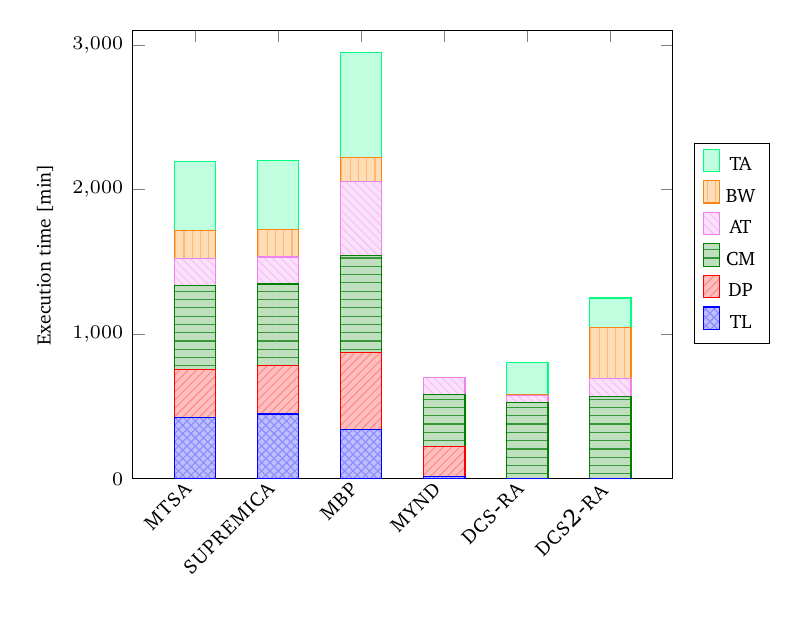
\begin{tikzpicture}
\begin{axis}[
  ybar stacked,
  bar width=15pt,
  enlarge x limits=0.15,
  ymin=0,
  ymax=3100,
  font=\scriptsize,
  xticklabel style={font=\small},
  reverse legend,
  legend style={at={(1.18,0.75)},legend columns=1},
  ylabel={Execution time [min]},
  symbolic x coords={\MTSA,\SUP,\MBP,\MYND,\RA,\RAnew},
  xtick=data,
  x tick label style={rotate=45,anchor=east},
  font=\fontsize{7}{7}\selectfont
]
\addplot+[ybar,color=blue,fill=blue!25,text=black,postaction={pattern=crosshatch,pattern color=blue!45}]
  plot coordinates {(\MTSA,421.93) (\SUP,448.3) (\MBP,341.31) (\MYND,15.58) (\RA,0.06) (\RAnew,0.34)}; % TL
\addplot+[ybar,color=red,fill=red!25,text=black,postaction={pattern=north east lines,pattern color=red!45}]
  plot coordinates {(\MTSA,331.49) (\SUP,334.62) (\MBP,534.78) (\MYND,211.14) (\RA,0.12) (\RAnew,0.15)}; % DP
\addplot+[ybar,color=Green,fill=Green!25,text=black,postaction={pattern=horizontal lines,pattern color=ForestGreen!90}]
  plot coordinates {(\MTSA,584.08) (\SUP,564.34) (\MBP,671.0) (\MYND,355.12) (\RA,525.24) (\RAnew,570.69)}; % CM
\addplot+[ybar,color=Violet,fill=Violet!25,text=black,postaction={pattern=north west lines,pattern color=Violet!50}]
  plot coordinates {(\MTSA,186.65) (\SUP,186.99) (\MBP,506.77) (\MYND,118.43) (\RA,52.80) (\RAnew,123.99)}; % AT
\addplot+[ybar,color=BurntOrange,fill=BurntOrange!25,text=black,postaction={pattern=vertical lines,pattern color=BurntOrange!55}]
  plot coordinates {(\MTSA,191.86) (\SUP,188.49) (\MBP,170.5) (\MYND,0.28) (\RA,1.66) (\RAnew,350.33)}; % BW
\addplot+[ybar,color=SpringGreen,fill=SpringGreen!25,text=black]
  plot coordinates {(\MTSA,480.91) (\SUP,477.1) (\MBP,721.8) (\MYND,0.48) (\RA,225.72) (\RAnew,205.13)}; % TA
\legend{\strut TL, \strut DP, \strut CM, \strut AT, \strut BW, \strut TA}
\end{axis}
\end{tikzpicture}
\end{figure}

\end{document}
